\section{Diagramas de Secuencia}
Los diagramas de secuencia fueron elaborados utilizando la herramienta {Visual Paradigm}~\cite{staruml2024}. La imagen \ref{DiagSec} muestra el diagrama de secuencia DS-001 correspondiente al caso de uso CU-001 Acceder al portal.

%%%%%%%%%%%%%%%%%%%%%%%%%%%

\begin{figure}[H]
    \centering
    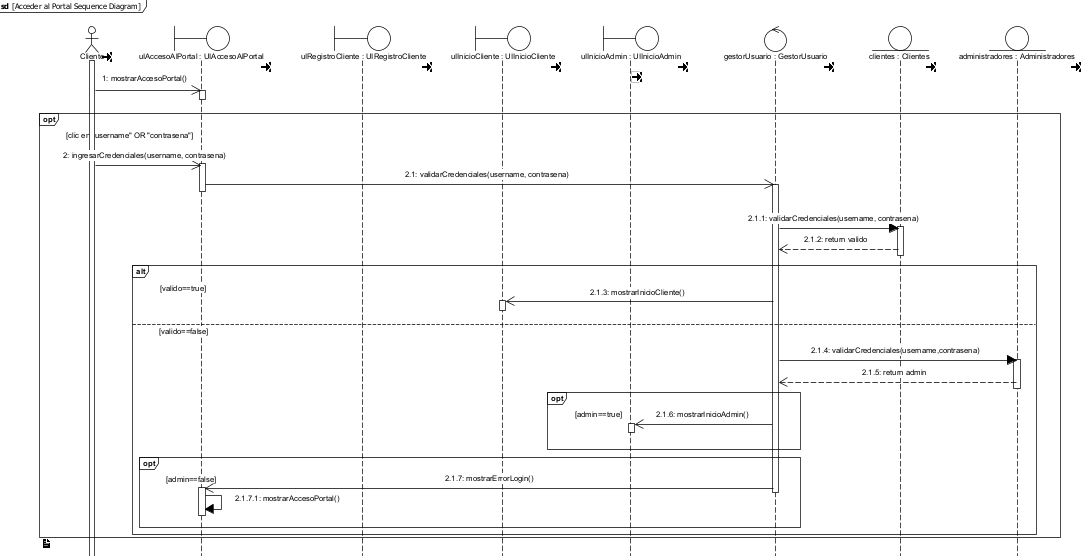
\includegraphics[width=0.95\linewidth]{Media/4_Disenio/CU-001_1.png}
    \caption{Diagrama de secuencia DS-001}
    \label{DiagSec}
\end{figure}

%%%%%%%%%%%%%%%%% 

\textbf{Link de acceso:} \linkDiagramaSecuencia \\

\textbf{Pasos de ejecución:}
\begin{enumerate}
    \item Ingresar al repositorio en GitHub usando el link proporcionado y descargar QCM.vpp.
    \item Abrir el archivo descargado en la herramienta Visual Paradigm.
    \item En la pestaña Diagram Navigator abrir UML Diagrams y en Sequence Diagram seleccionar el diagrama que se desea visualizar.
\end{enumerate}
\newpage